\section{Example 2: Security}

Security is defined as the ability of a system to withstand attacks. 
In contrast to safety, security does assume an adversary viciously attacking the software. 
%Being able to protect a system against attacks requires 
Developers need to anticipate and consider all potential attacks; in misuse-cases \cite{Alexander2002a}, this antagonism between two sides is made explicit. This \emph{externalization} is often supported by attack trees.%, which help developers to consider all possible attacks.

Knowledge about vulnerabilities, past attacks, and many other aspects of a software system is crucial for both sides. 
If developers want to stay ahead of attackers, they need to organize and use that knowledge. 
In the German DFG Priority Programme 1593 (Design for Future), we work on an approach for detecting vulnerabilities during requirements analysis. 
This ``SecVolution'' approach is fundamentally built on a knowledge-perspective of security \cite{Gaertner2014,fosad14}. 

Security is a quality aspect of growing importance: Large home entertainment systems may have been initially out of scope for security, but when they collect payment information or personal data, they suddenly become very security-relevant. 
Supermarket management software may start out as a local and non-distributed application of moderate size and limited security relevance. 
When an online-store component is added, software security definitely turns into a major concern. 
As these examples indicate, security is far from a commodity that can be added and removed at convenience. 
Instead, a single known vulnerability can make the entire system insecure. 
SecVolution investigates changes that can cause security to suffer. 
The above-mentioned scenarios exemplify this type of changes. 
However, there is an additional type of changes that is not mentioned above but just as severe: Even if nothing in the software changes, its security can suffer when attackers discover a new security breach in the existing code, and exploit it for an attack. 
A long-living system does not wear out over time, but it ages in relationship to the knowledge developers and attackers have about it. 
A core insight in SecVolution was how crucial it is to \emph{externalize} attacker and security knowledge from people; automate it in a tool, and help developers internalizing it when they see suspicious findings.


%Fig. Prinzipbild von SecVol
\begin{figure}
    \centering
    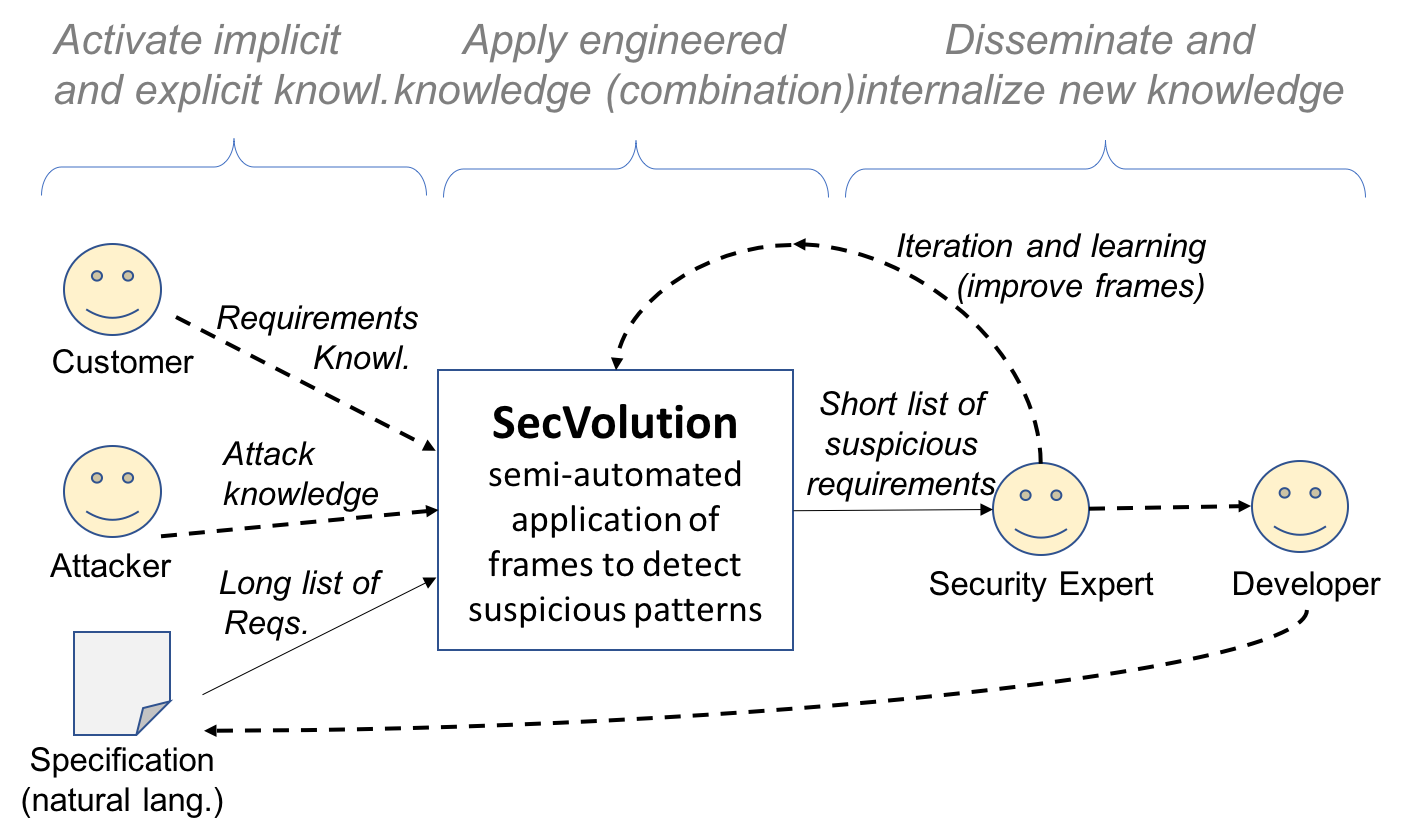
\includegraphics[width=\columnwidth]{figs/nnnOben}
    \caption{Three essential activities in managing knowledge on software quality attributes.}
    \label{fig:nnnOben}
\end{figure}

%We wanted to detect requirements that could introduce vulnerabilities. 
Highly qualified security experts are able to spot patterns of payment, data, access, and the like. 
However, those experts are rare and cannot check each and every document and use case. 
A presumably unproblematic system, such as a supermarket or smart TV, tends to be neglected in terms of security. 
Thus, SecVolution tries to detect as many known suspicious requirements and submit this much smaller list of requirements to the rare experts for final resolution. 
In order to extract knowledge from human-made natural language requirements, we use natural-language processing techniques. 
% About 79\% of requirements are still in natural language. 
After parsing the sentence grammatically, we search for matching Security Frames (i.e., suspicious patterns) and use an ontology to represent the knowledge. 


Techniques for soliciting and deriving explicit knowledge from  people who have internalized it can be very challenging \cite{Gaertner2014}. 
% Adding a new suspicious pattern to the heuristics could be done just in time. 
As a prerequisite, the %long-term 
collection of knowledge must be maintained as a long-term endeavor and the interplay of developers, attackers, and security experts must be investigated. 
